\section{MARCO TEÓRICO}
\subsection{SÍNTESIS DE FRECUENCIA}
Se puede construir un sintetizador de frecuencia alrededor de un PLL, tal como se muestra en la figura 1. Un divisor de frecuencia se inserta en la salida del VCO y el comparador de fase, para que la señal del lazo al comparador este a la frecuencia fo mientras que la salida es la fase del VCO es Nfo. Esta salida es un múltiplo de la frecuencia de entrada, pero siempre y cuando el lazo este en seguimiento. La señal de entrada puede salir de un oscilador a una f1, con la salida del VCO resultante en Nf1, si el lazo se ajusta para seguimiento a la frecuencia fundamental.

\begin{figure}[H]
    \centering
    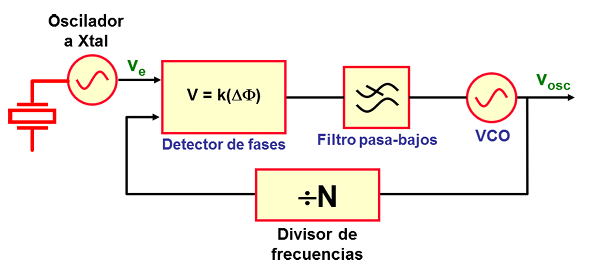
\includegraphics[width=.6\textwidth]{imgs/2.1. Esquemático de un sintetizador.png}
    \caption{Esquemático de un sintetizador}
\end{figure}

En esta experiencia se va a usar un PLL 565 como multiplicador de frecuencia y un 7490 como divisor. La entrada Vi a la frecuencia fo se compara con la entrada en el terminal 5. Una salida a Nfo que ahora es 10fo, se conecta para proporcionar la entrada en la terminal 14 al 7490, la cual varía ente -5 y +5 voltios. Con la salida en el terminal 9, que es la entrada al 7490 dividida entre 10, la señal del terminal del PLL es diez veces la frecuencia de entrada siempre y cuando el lazo permanezca en seguimiento. Debido a que el VCO puede variar solamente a lo largo de un rango limitado respecto a la frecuencia central, puede que sea necesario cambiar la frecuencia del VCO una vez que se cambie el valor del divisor.
\newpage
